\documentclass[12pt, oneside]{book}

% ~~~~~~~~~~~~~~~~~~~~~~~~~~~~~~~~~~~~~~~~~~~~~~~~~~~~~~~~~~~~~~~~~~~~~~~~~~~~~
%                                   IMPORTS
% ~~~~~~~~~~~~~~~~~~~~~~~~~~~~~~~~~~~~~~~~~~~~~~~~~~~~~~~~~~~~~~~~~~~~~~~~~~~~~
\renewcommand\figurename{Fig.}

\usepackage[a4paper, top=2.5cm, bottom=2.5cm, left=3.5cm, right=2cm]{geometry}
\usepackage[utf8]{inputenc}
\usepackage[slovak]{babel}
\usepackage{amsmath}

% enable including .pdf files, e.g. comenius logo (komlogo-new) and images
\usepackage{graphicx}
\usepackage{wrapfig}
\usepackage{natbib}
\usepackage{xcolor}
\usepackage{hyperref}
\usepackage{enumitem}
\hypersetup{
    colorlinks = true,
    linkbordercolor = black,
    linkcolor = red,
    citecolor = gray,
    urlcolor = blue,
}

% value 1.25 should correspond to 1.5 line spacing
\linespread{1.25}

\addto\captionsslovak{\renewcommand{\figurename}{fig.}}
\graphicspath{{pictures/}}
\bibpunct{(}{)}{;}{a}{,}{,}

% TODO:
% what are these used for?
% - \usepackage[hang, flushmargin]{footmisc}
% - \usepackage{pdfpages}
% - \usepackage{lmodern} % should be nicer font, but nothing changed...


% ~~~~~~~~~~~~~~~~~~~~~~~~~~~~~~~~~~~~~~~~~~~~~~~~~~~~~~~~~~~~~~~~~~~~~~~~~~~~~
%                             VARIABLE DEFINITIONS
% ~~~~~~~~~~~~~~~~~~~~~~~~~~~~~~~~~~~~~~~~~~~~~~~~~~~~~~~~~~~~~~~~~~~~~~~~~~~~~
\def\mfthesistype{Bachelor Thesis}
\def\mfauthor{Michal Hoľa}
\def\mfadvisor{Mgr. Peter Gergeľ}
\def\mfyear{2016}
\def\mfplacedate{Bratislava, \mfyear}
\def\programme{Applied Informatics}
\def\subject{9.2.9 \programme}
\def\department{Department of Applied Informatics}
\def\school{Comenius University in Bratislava}
\def\faculty{Faculty of Mathematics, Physics and Informatics}
\def\thesisname{
    Artifictial neural network as an opponent in Quoridor
}

\author{\mfauthor}
\title{\thesisname}
\date{\mfyear}

% ~~~~~~~~~~~~~~~~~~~~~~~~~~~~~~~~~~~~~~~~~~~~~~~~~~~~~~~~~~~~~~~~~~~~~~~~~~~~~
%                                DOCUMENT BODY
% ~~~~~~~~~~~~~~~~~~~~~~~~~~~~~~~~~~~~~~~~~~~~~~~~~~~~~~~~~~~~~~~~~~~~~~~~~~~~~
\begin{document}

  \input firstpages.tex
  \newpage

  \input abstract.tex
  \newpage

% ~~~~~~~~~~~~~~~~~~~~~~~~~~~~~~~~~~~~~~~~~~~~~~~~~~~~~~~~~~~~~~~~~~~~~~~~~~~~~
%                                   PREFACE
% ~~~~~~~~~~~~~~~~~~~~~~~~~~~~~~~~~~~~~~~~~~~~~~~~~~~~~~~~~~~~~~~~~~~~~~~~~~~~~

% ~~~~~~~~~~~~~~~~~~~~~~~~~~~~~~~~~~~~~~~~~~~~~~~~~~~~~~~~~~~~~~~~~~~~~~~~~~~~~
%                                   CONTENTS
% ~~~~~~~~~~~~~~~~~~~~~~~~~~~~~~~~~~~~~~~~~~~~~~~~~~~~~~~~~~~~~~~~~~~~~~~~~~~~~

% ~~~~~~~~~~~~~~~~~~~~~~~~~~~~~~~~~~~~~~~~~~~~~~~~~~~~~~~~~~~~~~~~~~~~~~~~~~~~~
%                                 INTRODUCTION
% ~~~~~~~~~~~~~~~~~~~~~~~~~~~~~~~~~~~~~~~~~~~~~~~~~~~~~~~~~~~~~~~~~~~~~~~~~~~~~
  \section{Introduction}
    \subsection{Quoridor Rules}

    \begin{wrapfigure}{R}{0.4\textwidth}
      \vspace*{-0.48cm}
      \centering
      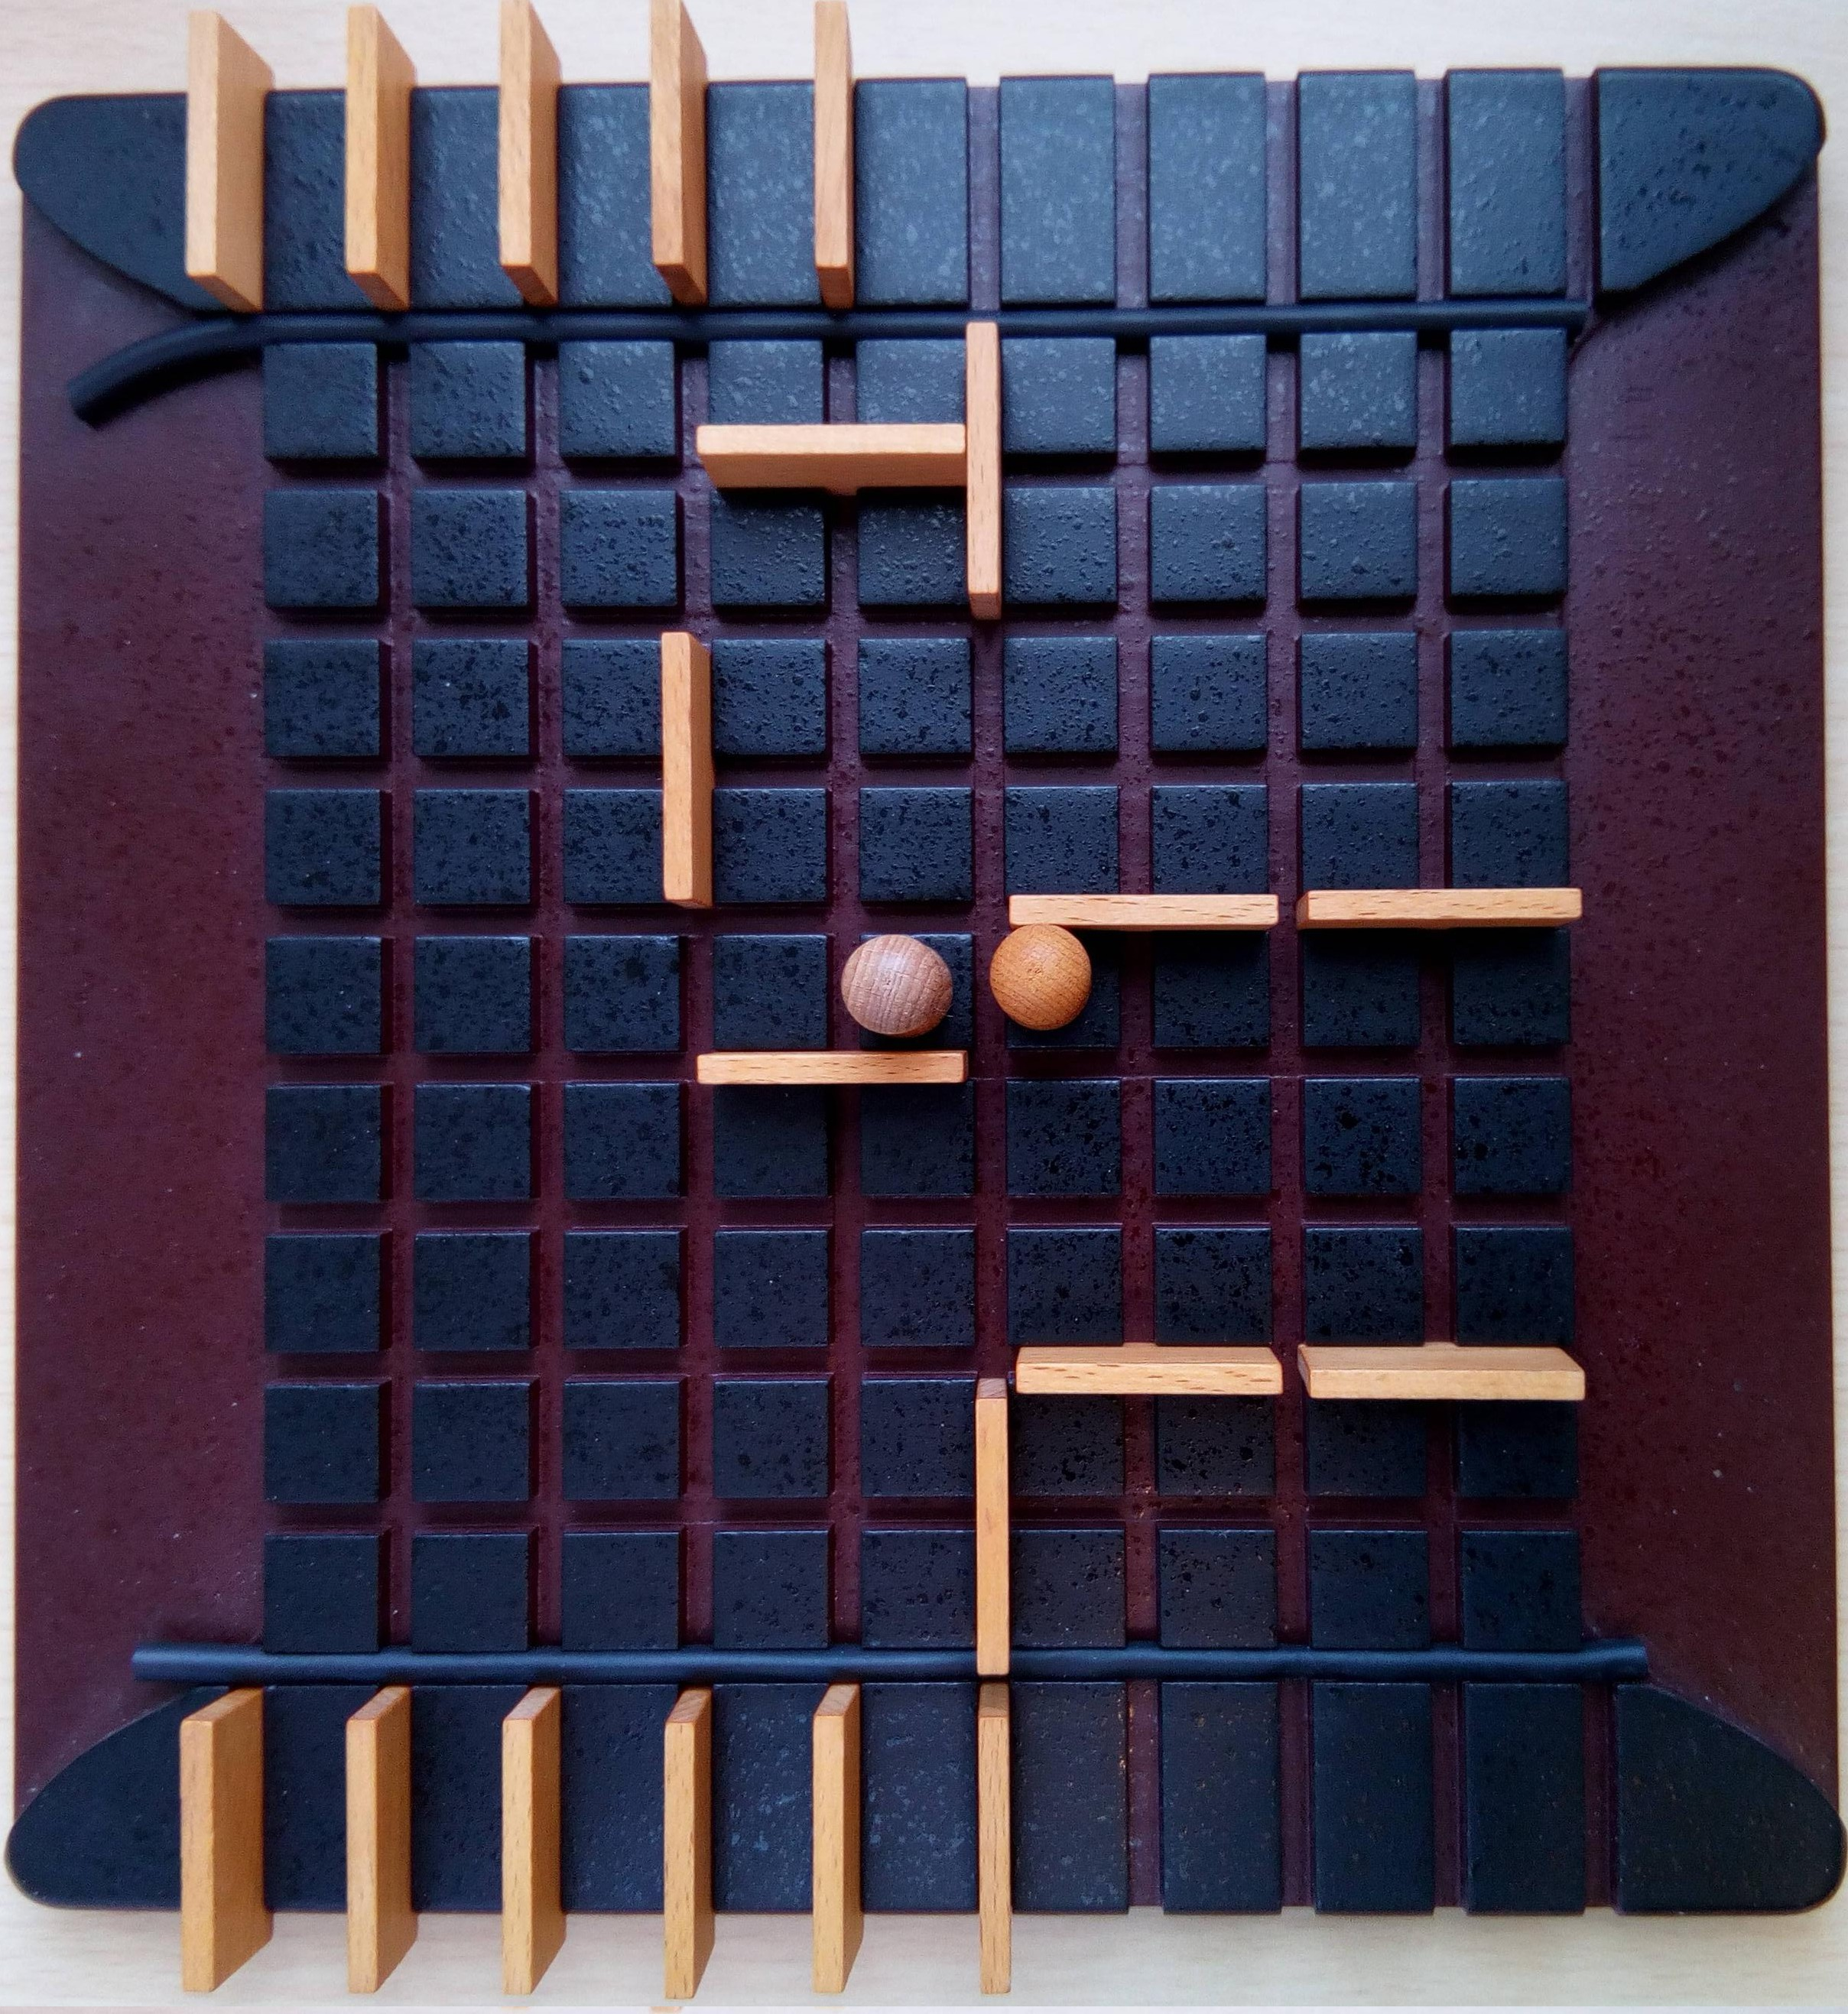
\includegraphics[width=0.35\textwidth]{real_board.jpg}
      \vspace*{-0.60cm}
      \caption{real board}
      \label{fig:real_board}
      \vspace*{-0.60cm}
    \end{wrapfigure}

    Quoridor is abstract board strategy game for 2 or 4 players with size of
    9x9 (81) squares. This thesis covers 2 player version of this game.

    \begin{wrapfigure}{R}{0.4\textwidth}
      \vspace*{-0.98cm}
      \centering
      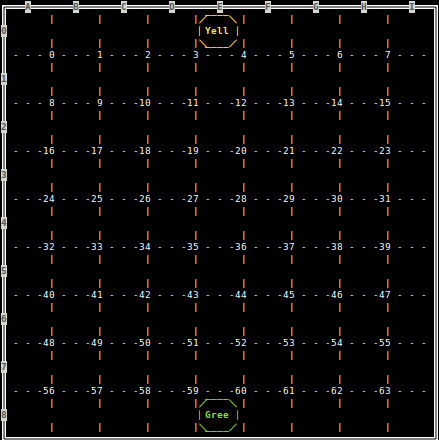
\includegraphics[width=0.35\textwidth]{start.png}
      \vspace*{-0.60cm}
      \caption{game start}
      \label{fig:game_start}
      \vspace*{-1.40cm}
    \end{wrapfigure}

    Each player starts with a single pawn in the center of the edge on the
    opposite side as the opponent.
    The goal for each player is to reach the opposite edge.

    Player also starts with 10 walls (fences) in the stock.
    Walls are two space wide and can be placed in the groove that runs between
    the spaces.
    Placed wall blocks pawns paths forcing them to go arount it.
    Walls once placed can not be moved nor removed.
    Wall can not be placed to the position already occupied or crossing by
    other wall.
    Also, wall can not cut off the only remaining path of any pawn to his goal.

    When player is on turn, he must place wall, if he has left some, or move
    his pawn to adjacent (not diagonal and unoccupied) space.
    If opponent's pawn stands on an adjacent space, current player can jump
    with his pawn to all the places where the opponent pawn can move.

  \subsection{Q-Learning}
    Q-Learning is reinforcement learning method. It learns an action-value
    (q-value) function for any finite Markov decision process used to find
    optimal policy for the agent. After it has learned the q-value function,
    it can follow the optimal strategy by choosing best q-value. ?citation?
    Algorithm is value iteration update for every observed state ?citation?:
    \begin{equation}
    Q_{t+1} \leftarrow Q_t(s_t, a_t) + \alpha \cdot (
        R_{t+1} + \gamma\cdot {\max_a}\,Q_t(s_{t+1}, a) - Q_t(s_t, a_t)
    )
    \end{equation}
    where $Q_t(s_t, a_t)$ is old value, $\alpha$ is learning rate, $R_{t+1}$ is
    reward after performing action $a_t$ in state $s_t$, $\gamma$ is discount
    factor and $\underset{a}{\max}\,Q_t(s_{t+1}, a)$ is maximum optimal future
    value.
    \newpage

  \subsection{Quoridor complexity}
    \begin{wrapfigure}{r}{0.5\textwidth}
      \vspace*{-1.45cm}
      \begin{equation}
        \label{eqn:mertensestimate}
        \begin{aligned}
          S_p &= 81 \cdot 80 = 6480
          \\
          S_f &= \sum_{i=0}^{20}\prod_{j=0}^{i}(128 - 4i) = 6.1582\cdot10^{38}
          \\
          S &= S_p \cdot S_f = \mathbf{3.9905 \cdot 10 ^{42}}
        \end{aligned}
      \end{equation}
      \vspace*{-1.45cm}
    \end{wrapfigure}

    Estimated game state complexity was $3.9905\cdot10^{42}$
    [\cite{mertens} (2)], however, this is very rough estimate, since it
    includes many states multiple times, since it counts with permutations
    instead of combinations of walls.
    % of walls which should be corrected to $
        % $\underset{j=0}{\overset{i}{\prod}}{128 \choose {128 - 4i}}$
        % S_f\!=\!\underset{i=0}{\overset{20}{\sum}}
        % \underset{j=0}{\overset{i}{\prod}}
        % {128 \choose {128 - 4i}}
    % $.

    My approach with estimate will be similar. I will estimate maximum states
    of this game, which will include impossible states such as:
    \begin{enumerate}[topsep=0pt,itemsep=-1ex,partopsep=1ex,parsep=1ex]
      \setlength\itemsep{0em}
      % \item both pawns in the winning positions
      \item pawn in the winning position where it could not end due to walls
      \item pawns not having the path to the winning position
      \item walls crossing each other
      \item pawn in the winning position and on turn
    \end{enumerate}
    Moreover, this estimate will it count as a different state when different
    player is on the move and also different number of walls in players stocks.
    Both of these could make the game very different in the outcome.

    \begin{wrapfigure}{r}{0.5\textwidth}
      \vspace*{-1.45cm}
      \begin{equation}
        \label{eqn:correctsp}
        \begin{aligned}
          S_p &= 81 {\cdot} 80 - 9 {\cdot} 9 = 6399
          \\
          f(i)&= \begin{cases}
            i + 1  & \quad \text{if } i <= 10 \\
            21 - i & \quad \text{if } i > 10
          \end{cases} \\
          S_f &= \sum_{i=0}^{20} f(i){128 \choose i} = 1.7796 {\cdot} 10^{23}
          \\
          S &= 2 {\cdot} S_p {\cdot} S_f = \mathbf{2.2775866 {\cdot} 10^{27}}
        \end{aligned}
      \end{equation}
      \vspace*{-0.45cm}
    \end{wrapfigure}
    $S_p$ was corrected to not include both pawns in the winning positions.
    $f(i)$ % is from sequence $\{1, 2, ..., 9, 10, 11, 10, 9, ..., 2, 1\}$ and
    stands for different wall counts in the stocks.
    $2$ in $2{\cdot} S_p {\cdot} S_f$ counts different players on turn.

    Result is maximum number of states, which is significantly less then former
    estimate. However, even if I could evaluate $10^{6}$ states in one second,
    it would take around $7.2172{\cdot}10^{13}$ years to evaluate this many
    states. Also, lets assume it takes on average 50B of memory per state. Then
    I would need approximately $1.138793{\cdot}10^{29}$ bytes of memory to
    store all states in the computer.

  \subsection{Perceptron}

    \begin{wrapfigure}{l}{0.4\textwidth}
      \vspace*{-0.45cm}
      \centering
      \includegraphics[width=0.4\textwidth]{neural-net1.png}
      \vspace*{-1.45cm}
      \caption{ANN}
      \label{fig:network}
      \vspace*{-1.00cm}
    \end{wrapfigure}

    Artifitial neural network (ANN) is a family of models inspired by biological
    neural networks used in computer science to approximate functions with
    large number of inputs. Generally, artifitial neural network is presented
    as a system of interconnected neurons exchanging messages between each
    other. These connections have weights that can be adjusted based on
    experience which makes the network capable of learning.

    Perceptron is an algorithm for supervised learning of binary classifiers
    where one neuron has multiple weighted inputs and single output. Single
    perceptron can learn to decide between two linearly separable
    classes. Multiple perceptrons in multiple layers (MLP) use arbitrary
    activation function which makes it able to perform classification or
    regression based on the activation function chosen.

\renewcommand\bibname{References}
\bibliographystyle{plainnat}
\bibliography{references}

\end{document}
